\section{Experiments}
\label{Sec:Experiments}

% This section evaluate Cerberus by answering several key questions.
% \begin{itemize}
%         \item \textbf{Q1}: will Cerberus improve application performance
%                 by utilizing burst buffer nodes?
%         \item \textbf{Q2}: Will job demand on burst buffer affect Cerberus?
%                 Why bother to divide the job execution into 3 phases?
%         \item \textbf{Q3}: Can dynamic programming based optimization
%                 help Cerberus further
% improve application performance?
% \end{itemize}
% Our newly developed event-driven simulator, BBSim, is used to simulating
% the Trinity system described later.

%==============XY===================
This section evaluate Cerberus by answering 3 key questions.
\begin{itemize}
        \item \textbf{Q1}: Will utilizing burst buffer nodes 
        improve both jobs and system performance?
        \item \textbf{Q2}: Will job demand on burst buffer affect Cerberus?
                Why bother to divide the job execution into 3 phases?
        \item \textbf{Q3}: Can dynamic programming based optimization
                makes Cerberus even better?
\end{itemize}
We integrate Cerberus into our newly developed event-driven simulator, 
BBSim, and evaluate Cerberus against the traditional FCFS/EASY backfilling scheduler.
Codebase of BBsim and Cerberus are public to the community
\footnote{Available at https://github.com/urlplaceholder}.
% metric

% We select two evaluation metrics, job's \textit{response time} and 
% \textit{system throughput}, when evaluating our design.
% Response time is the time duration from job submission to its fully completion,
% which is the major concern from user's perspective.
% On the other hands, system throughput, defined as the number of jobs finished in
% a fixed time period (500 seconds), measures the performance of computing system.

%==============XY===================
We select three evaluation metrics, job's \textit{response time}, \textit{wait time} and 
\textit{system throughput}, when evaluating our design.
Response time is the time duration from job submission to its fully completion,
which is the major concern from user's perspective.
Wait time is the aggregated time a job waits in each queue.
System throughput, defined as the number of jobs finished in
a fixed time period (500 seconds), measures the performance of the system.


\subsection{Simulation Settings}
% % system
% We consider simulating the full Trinity super computer\cite{TrinitySystem}.
% The number of compute nodes on Trinity is about 18,936,
% e.g. 9,436 Intel Haswell nodes
% and at least 9500 Intel Xeon Phi nodes.
% There are 16 cores on each processor, thus totally 302,976 cores.
% In the following experiments, we compare two identical system except that
% IO nodes are replaced by the same number of burst buffer nodes.
% Eventually Trinity plans to delivery up to 576 burst buffer nodes of 3.7 PB,
% consisted of Trinity IO nodes with PCIe SSD card.
% They are globally accessible as intermediate storage and distributed among cabinets.
% Sequential read/write speed of burst buffer nodes is 8.0 GBps.
% Bandwidth between CPU node and non-burst-buffer IO node is set to 2.5 GBps.


We simulate a burst buffer enabled system as shown in Figure~\ref{Fig:BBArchitecture}.
This system architecture is inspired by Trinity~\cite{TrinitySystem}, 
the next generation supercomputer in Los Alamos National Laboratory.
The parameters used in our simulation are taken from their technique report\cite{BBUseCase}.
The simulated system consists of 18,936 compute nodes,
e.g. 9436 Intel Haswell nodes and 9500 Intel Xeon Phi nodes.
There are 576 burst buffer nodes with aggregated 3.7 PB storage capacity, 
which are globally accessible as intermediate storage.
Sequential read/write speed of burst buffer nodes is 8.0 GBps.
Bandwidth between CPU node and IO node is set to 2.5 GBps.

\begin{figure}[!t]
        \centering
        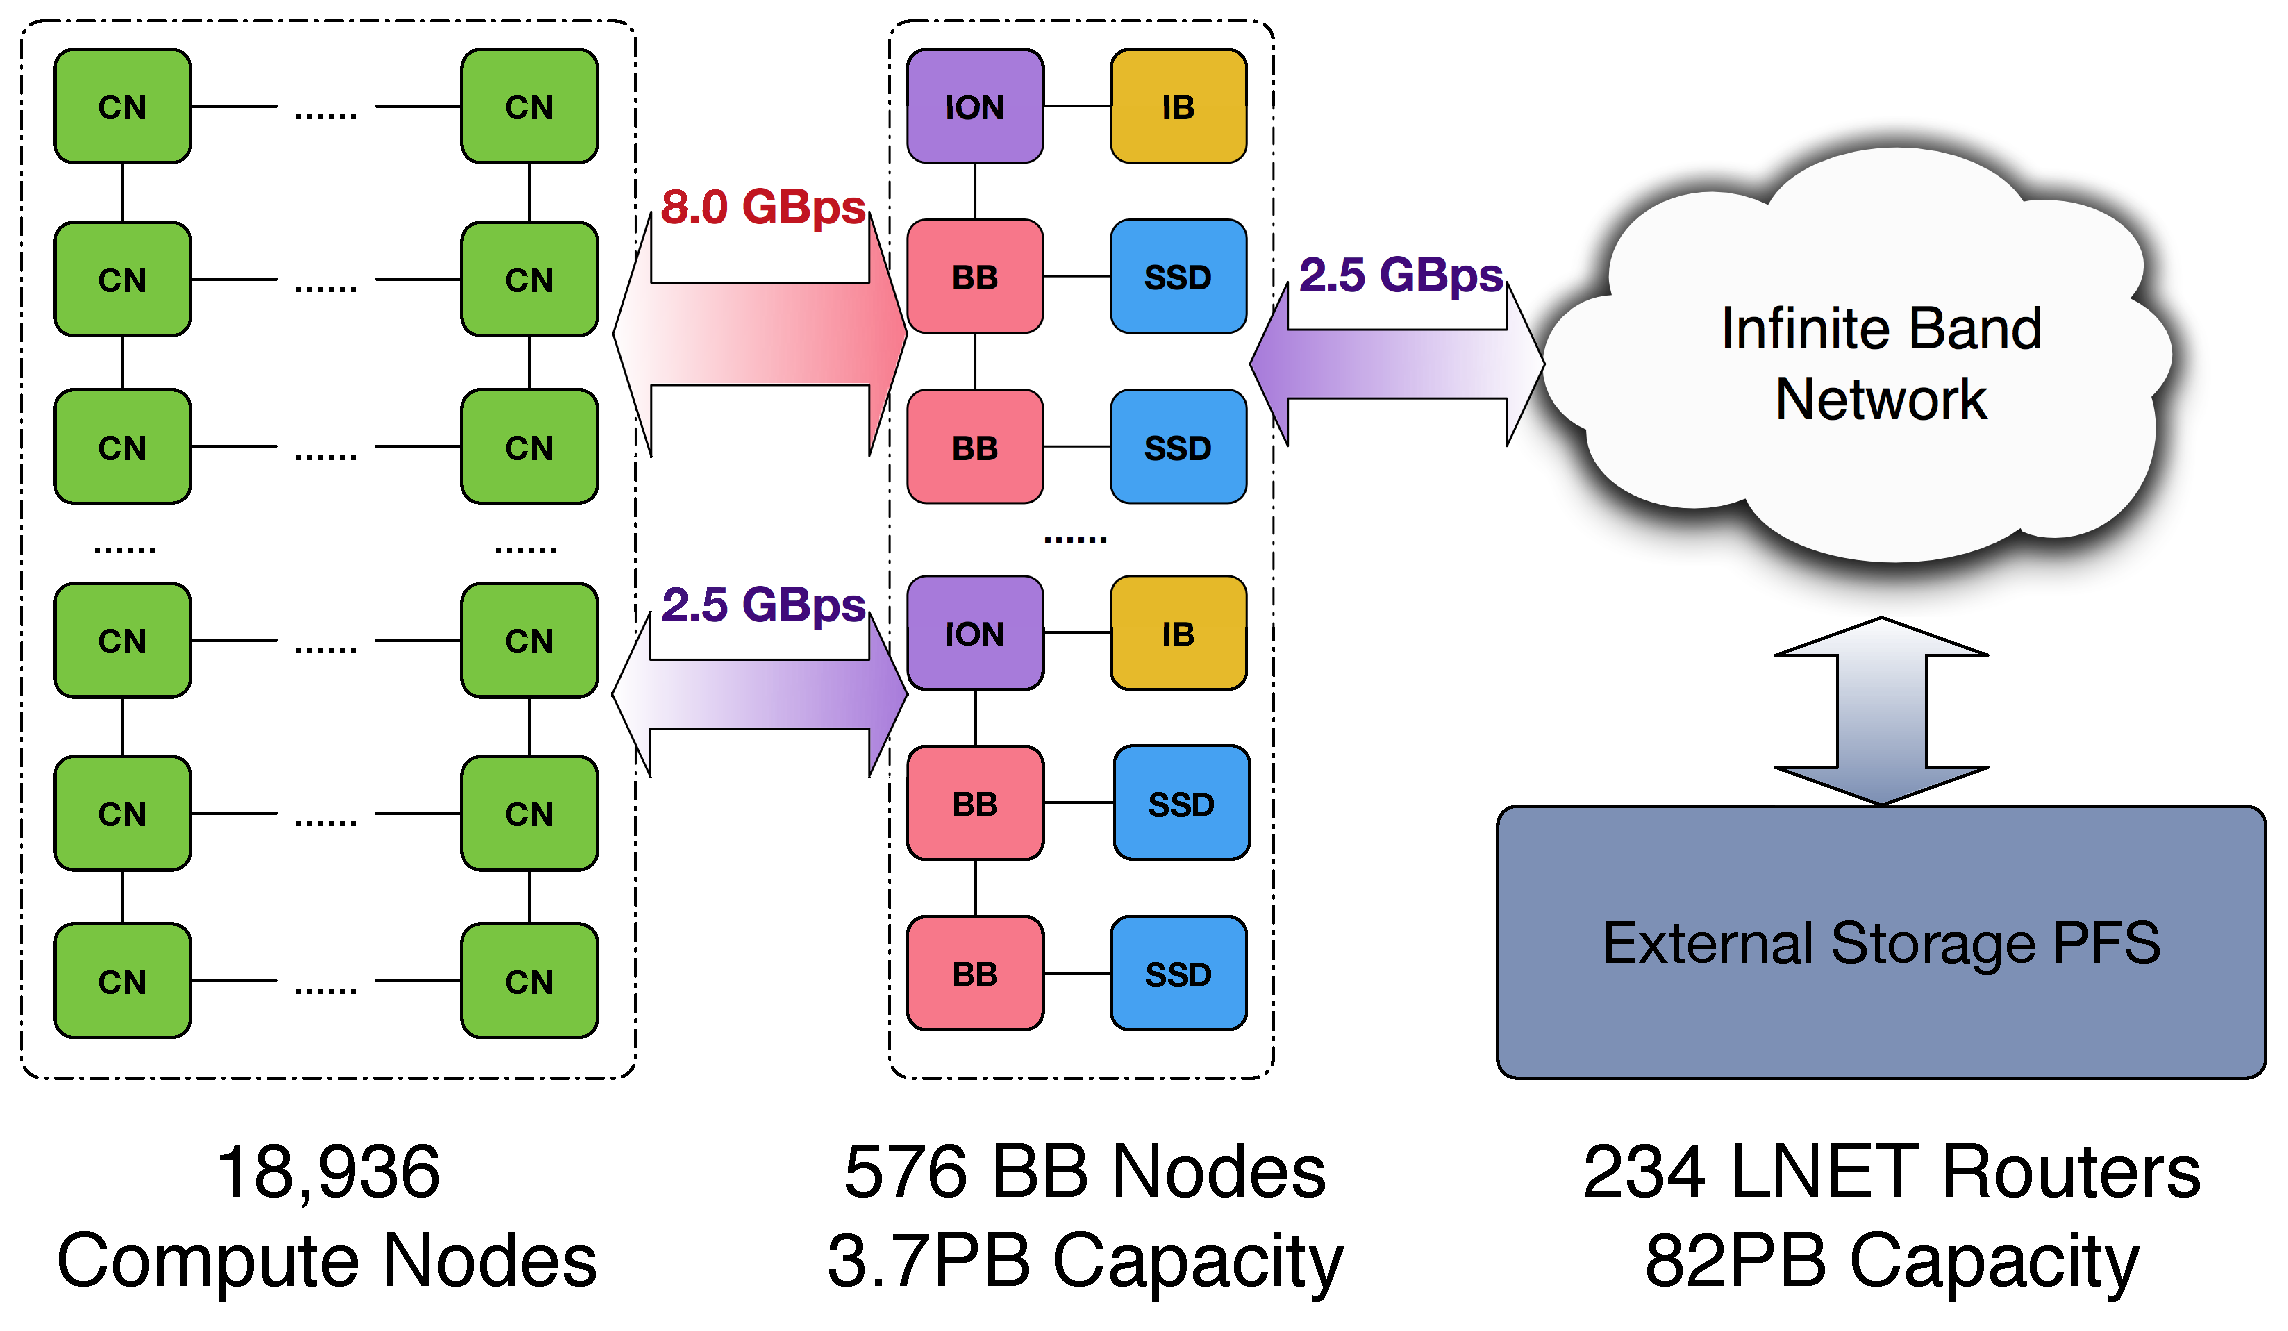
\includegraphics[width= 3.5in]{BBArchitecturewithBandwidth}
        \caption{Overview of Simulated System: A Burst Buffer Enabled Supercomputer Inspired by Trinity}
        \label{Fig:BBArchitecture}
\end{figure}

% % trace
% Job trace is from ANL's Blue Gene Intrepid system,
% containing totally 68,936 jobs run during January to September 2009\cite{JobTrace}.
% We extract two critical fields from this jobs trace: running time and
% number of cores user requested.
% In this section we take a window of 1,185 jobs and report their scheduling results.
% We patched 3 fields to each job's log entry: the amount of input data $data\_in$,
% the total amount of written data for checkpointings $data\_run$
% and the amount of output data $data\_out$.
% We assume $data\_run$ and $data\_out$ follows uniform distribution with
% lower boundary of 1 TiB and upper boundary of 60 TiB;
% $data\_in$ follows uniform distribution between 1 GiB and 30 Gib.
% The patches 3 fields may or may not be used in scheduling,
% depends on both the model of the jobs and the experiment scenario.


Since Trinity is not ready for the time being, there is no Trinity job log available for our study.
We use the job log collected from ANL's Blue Gene Intrepid system. The log contains 68,936 jobs
submitted to the system from January to September 2009~\cite{JobTrace}.
We patched 3 fields to each job's log entry: the amount of input data $data\_in$,
the total amount of written data for checkpointings $data\_run$
and the amount of output data $data\_out$.
We assume $data\_run$ and $data\_out$ follows uniform distribution with
lower boundary of 1 TiB and upper boundary of 60 TiB;
$data\_in$ follows uniform distribution between 1 GiB and 30 Gib.



% \subsection{BB-Enabled System v.s. IO-Node-Only System}
\subsection{Utilizing BB v.s. Direct IO}
\label{Sec:Sim:DirectIOvsBB}
% In this section, we demonstrate that by utilizing burst buffer nodes,
% job scheduler could improve the performance of both applications and system.
% We compare two systems:
% \begin{itemize}
%         \item \textbf{1-Phase IO}: system without burst buffer nodes
%                 scheduled by FCFS policy
%         \item \textbf{Cerberus}: system with burst buffer 
%                 scheduled by our proposed Cerberus
% \end{itemize}


%=============XY==============

PFS is mounted by all compute nodes in the Trinity architecture, thus applications have the
option to bypass the burst buffer and use the file system directly for their IO operations. 
We refer this scenario as \textit{Direct IO}. Apparently, the performance of \textit{Direct IO}
is limited by the low dandwidth of IO nodes. However, applications will be exempted from 
waiting in the stage-in/out phases in the case of \textit{Direct IO} rather than utilizing burst buffer.
In this section, we compare the performance of applications utilizing burst buffer
against \textit{Direct IO}.
Based on the comparison, we answer question \textbf{Q1}: by utilizing burst buffer nodes,
both the performance of jobs and system can be greatly improved. 


% Figure~\ref{Fig:DirectIOvsBBResponse} compares CDF of the response time of 1185 jobs.
% When scheduler can allocate burst buffer to jobs,
% response time is bounded by 376,443.12 seconds.
% However, the worst case in system without burst buffer
% (Direct IO) is catastrophical.
% There are jobs that takes 889,239.20 seconds to finish,
% which is 2.36 times slow as the most non-responsive job
% in system equipped with burst buffer.
% In average case, \textit{nearly 99\% of the jobs scheduled by Cerberus
% response faster than Direct batch scheduler on non-BB system.}
% The improvement mainly comes from the difference of IO operation efficiency between
% traditional IO nodes and burst buffer nodes.

%=============XY==============
Figure~\ref{Fig:DirectIOvsBBResponse} compares CDF of jobs response
time by on burst buffer enabled system and the traditional system (Direct IO).
When running on system with burst buffer,
jobs response time is bounded by 376,443.12 seconds.
However, the worst case of Direct IO is catastrophic.
There are jobs that takes 889,239.20 seconds to finish,
which is 2.36 times slow as the most non-responsive job
in system equipped with burst buffer.
In average case, \textit{nearly 99\% of the jobs scheduled on the burst buffer enabled system
response faster than the traditional system without burst buffer.}
The improvement is intuitive, since the burst buffer can mitigate the IO gap between
IO nodes and compute nodes.


% Figure~\ref{Fig:DirectIOvsBBWait} reveals the total waiting time for both cases.
% Notice that system without burst buffer only request compute nodes.
% In this case, waiting time is the duration from its submission
% to actual starting running.
% The difference of worst case waiting time is drastic.
% Without burst buffer nodes, job's wait duration in worst case is 3.02 times
% slow as the worst one on systems with burst buffer;
% the upper bound of waiting duration for burst buffer systems is about 285,254 seconds.
% Because of burst buffer's better ability to
% absorb checkpoint operations and data moving in/out,
% the execution pipeline of job series is significantly speed up.
% Statistically, \textit{more than 80\% jobs waited less time, thus response faster,
% if they can access burst buffer.}

%=============XY==============
Figure~\ref{Fig:DirectIOvsBBWait} reveals jobs aggregated waiting time.
Noticing that in the case of Direct IO, jobs only request compute nodes.
Thus, waiting time is the duration between submission
and starting to run.
The difference of worst case waiting time is drastic.
On the system without burst buffer nodes, job's wait duration in worst case is 3.02 times
slow as the worst one on the burst buffer enabled system;
the upper bound of waiting duration for burst buffer systems is about 285,254 seconds.
Because of burst buffer's better ability to
absorb checkpoint operations and data moving in/out,
the execution pipeline of job series is significantly speed up.
Statistically, \textit{more than 80\% jobs waited less time, thus response faster,
if they can access burst buffer.}

% Using the collected completion time, we calculate system's throughput over time sequence.
% Figure~\ref{Fig:DirectIOvsBBThroughput} shows the system throughput for
% both system using burst buffer nodes and not.
% As indicated by the bar chart,
% \textit{the ratio of average throughput between two systems is 2.36},
% namely 1.575 to 0.667.
% It totally takes 889,239 seconds for the system without burst buffer nodes to
% server all 1185 jobs.
% The last job is job \#1150, which requested 4096 cores and 59 TB data space.
% It starts at 1126 seconds but waited 827,241 seconds.
% In contrast, when system installed burst buffer nodes,
% it accomplishes the same 1185 jobs in 376,443 seconds.
% Job \#1150 is the second last job finished, but both its waiting time and response time
% are significantly reduced, 272,741 and 376,026 seconds respectively.

%=============XY==============
Figure~\ref{Fig:DirectIOvsBBThroughput} shows the system throughput for
both system using burst buffer nodes and not.
As indicated by the bar chart,
\textit{the ratio of average throughput between two systems is 2.36},
namely 1.575 to 0.667.
It totally takes 889,239 seconds for the system without burst buffer nodes to
complete the workload.
We pick a specific job, job with ID \#1150 from the workload, to observe its
waiting time in both cases.
Job \#1150 request 256 compute nodes and 59 TB data space.
It starts at 1126 seconds but waited 827,241 seconds.
In contrast, when system installed burst buffer nodes,
it accomplishes the same workload in 376,443 seconds, and waiting time and response time of job \#1150
are significantly reduced, 272,741 and 376,026 seconds respectively.


\begin{figure*}[!t]
        \centering
        \subfloat[Job Response Time] {
                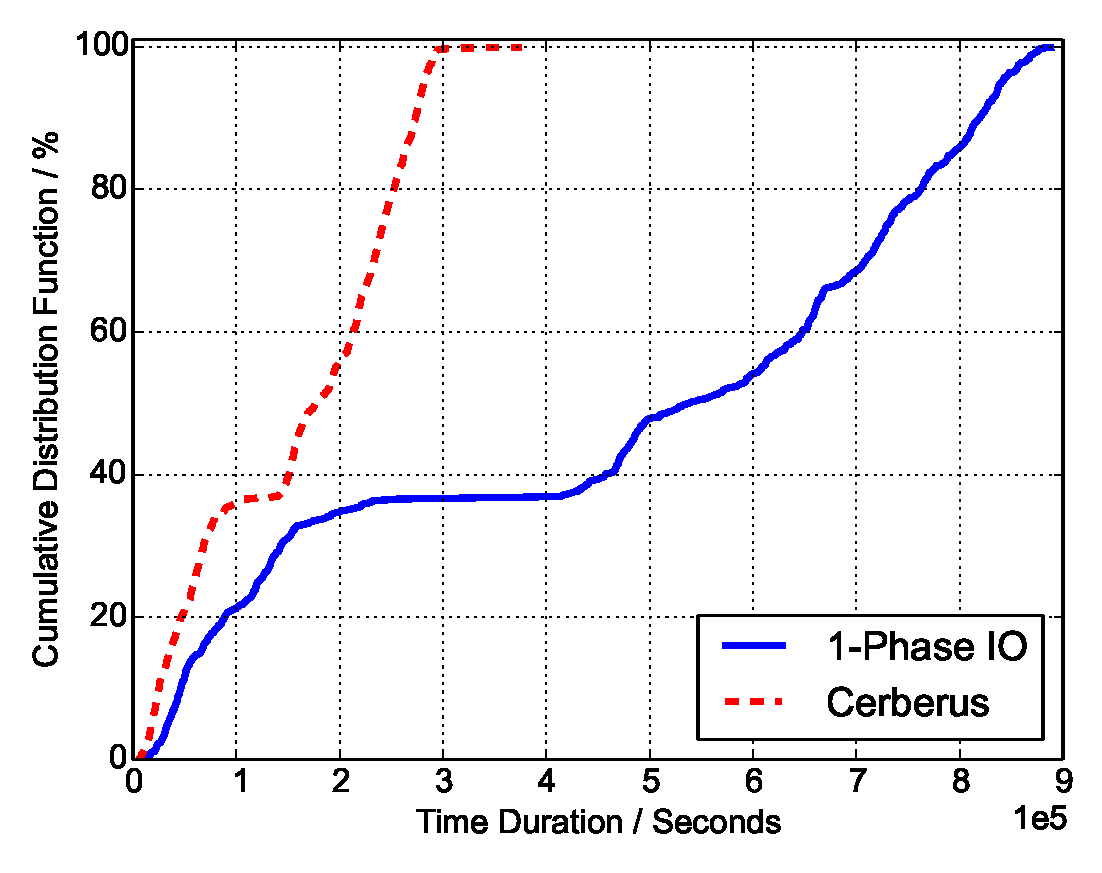
\includegraphics[width=2.2in]{IOvsBBFigures/1000jobs_direct_vs_bb_response}
                \label{Fig:DirectIOvsBBResponse}
        }
        \subfloat[Job Wait Time] {
                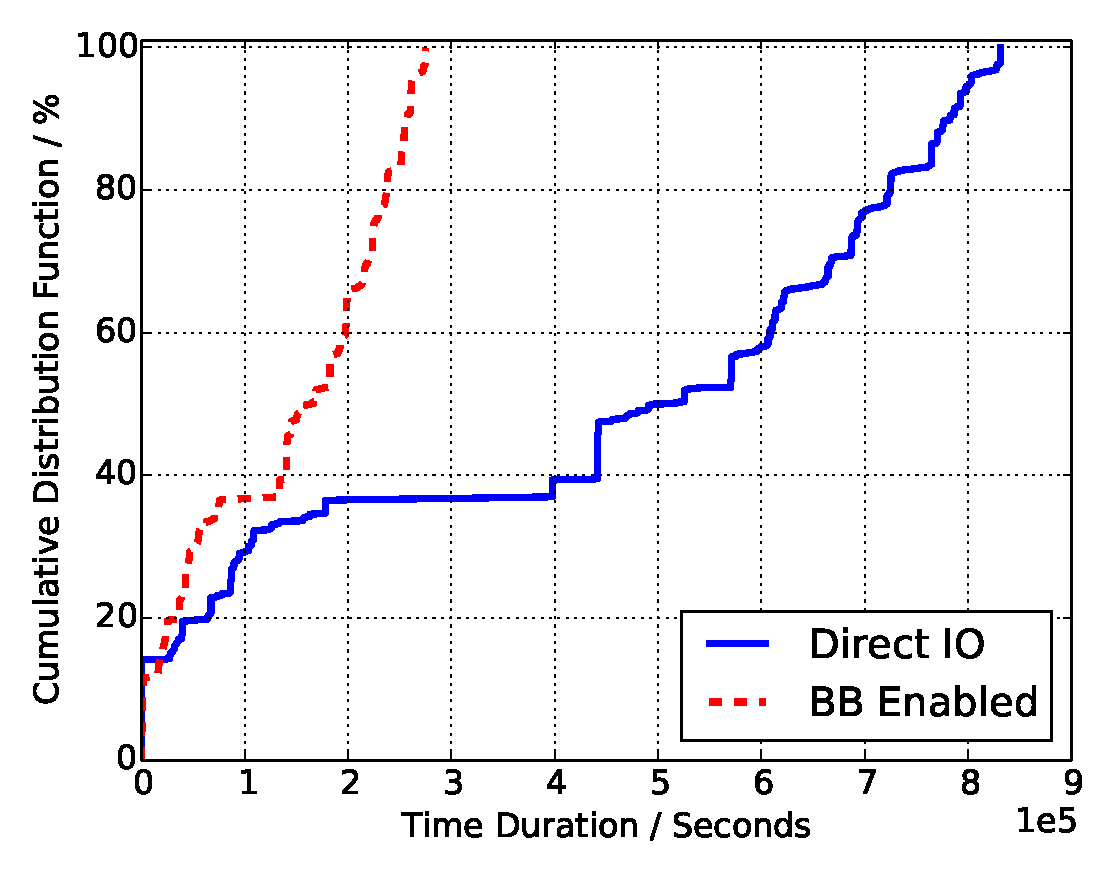
\includegraphics[width=2.2in]{IOvsBBFigures/1000jobs_direct_vs_bb_wait}
                \label{Fig:DirectIOvsBBWait}
        }
        \subfloat[System Throughput] {
                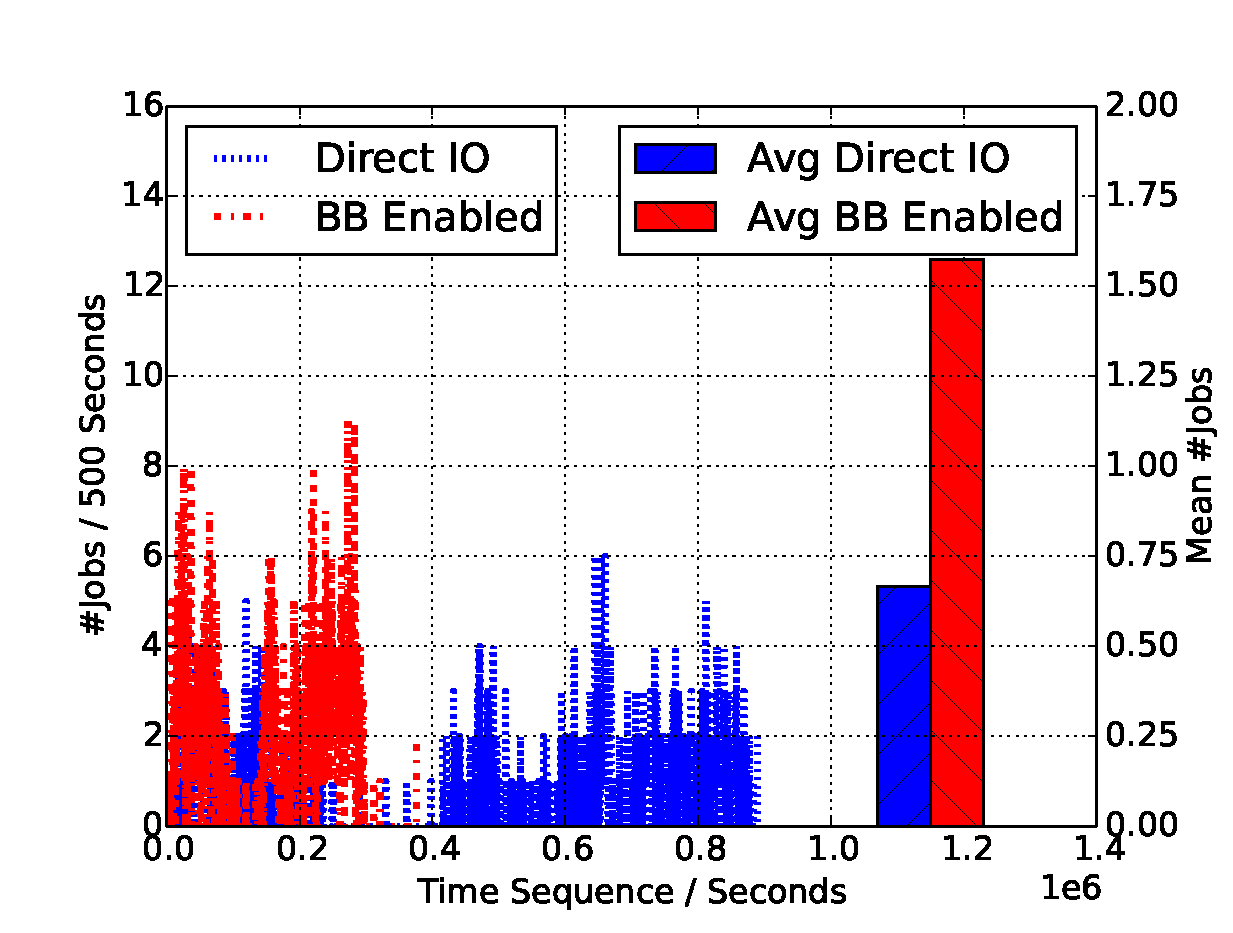
\includegraphics[width=2.5in]{IOvsBBFigures/1000jobs_direct_vs_bb_throughput}
                \label{Fig:DirectIOvsBBThroughput}
        }
        \caption{Utilizing Burst Buffer v.s. Direct IO}
        \label{Fig:DirectIOPerformance}
\end{figure*}

%\begin{figure}[!t]
        %\centering
        %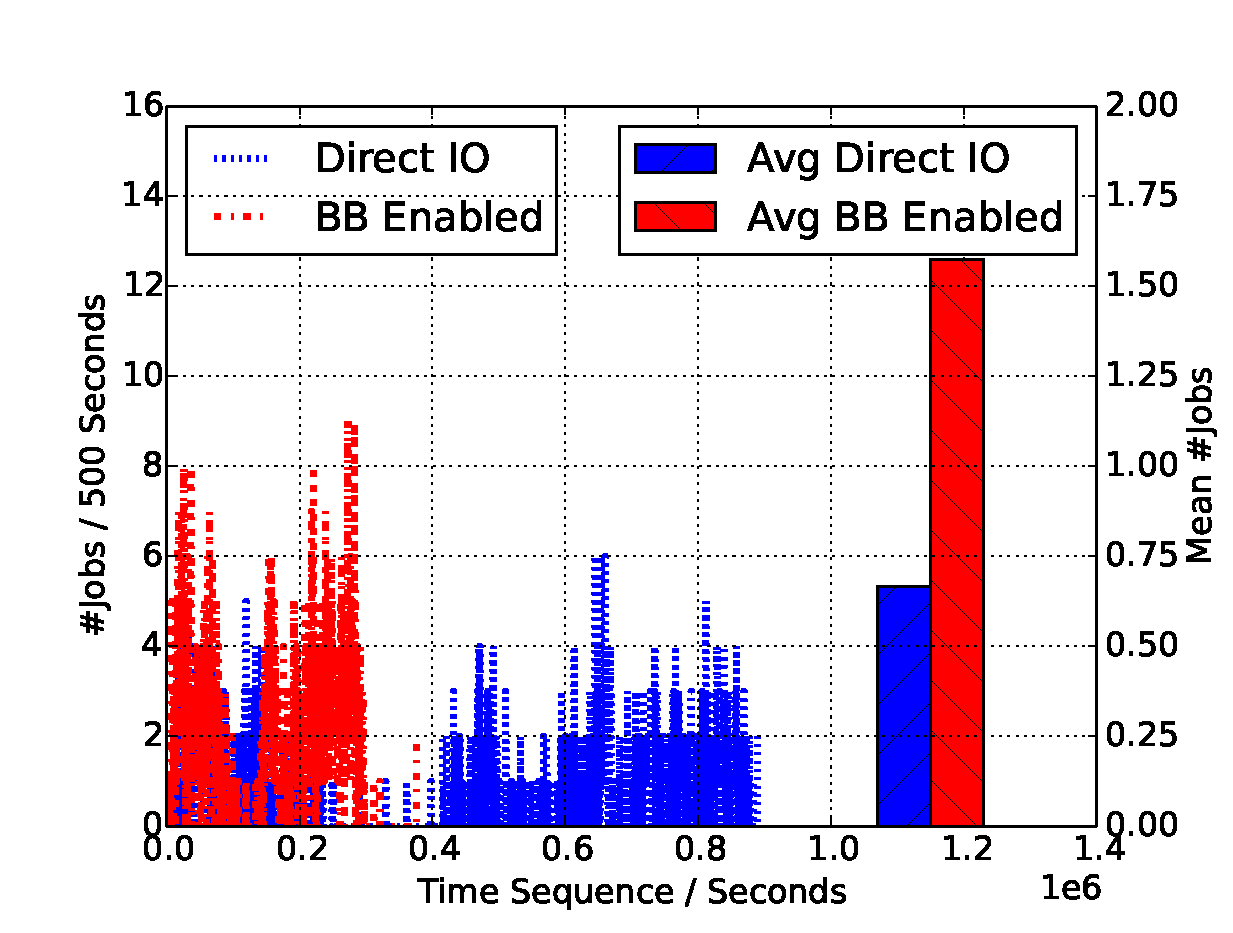
\includegraphics[width=3.2in]{IOvsBBFigures/1000jobs_direct_vs_bb_throughput}
        %\caption{System Throughput, IO Node Only vs. Burst Buffer System}
        %\label{Fig:DirectIOvsBBThroughput}
%\end{figure}


\subsection{3-Phase Model v.s. 1-Phase Model}
In this section we validate our 3-phase model by answering question \textbf{Q2}.
Simulation results demonstrate that jobs performance are improved 
when the scheduler makes scheduling decision in each phase separately.
Thus users are encouraged to provide detailed burst buffer demand in each phase for their jobs.

% In Figure~\ref{Fig:3Pvs1PResponse}, we plot 3 different scheduling results by 3 FCFS scheduler.
% \begin{itemize}
%         \item \textbf{1-Phase BB}: Jobs are modeled as just 1 phase.
%                 Users just provide general burst buffer demand throughout
%                 entire application lifetime.
%         \item \textbf{1D Cerberus}: In this case Cerberus only knows
%                 the overall burst buffer demand.
%         \item \textbf{Cerberus}: Users kindly provided all the burst buffer
%                 demand in all 3 phases.
%                 %the same as Cerberus in section~\ref{Sec:Sim:DirectIOvsBB}
% \end{itemize}
% We simulate the 3 cases with the same generated random data volume sequence.
% We assume the overall burst buffer demand in 1-phase BB and 1D Cerberus is
% $\max \{data\_in, data\_out, data\_run\}$.
% Notice that 1-phase BB scheduler must subject to burst buffer capacity constraint.
% %For 1-phase-modeled jobs, scheduler will make decision
% %based on $\max \{data\_in, data\_out, data\_run\}$
% %since we assume user will only tell the upper bound of its application's demand.
% %However, in simulation, we use the generated data amount as the same as 3-modeled jobs.
% %Response time of system without burst buffer devices are also plotted for comparison.

%========XY========================
In Figure~\ref{Fig:3Pvs1PResponse}, the scheduling results are based on three models
are presented:
\begin{itemize}
        \item \textbf{1-Phase-1D}: Jobs are submitted with total burst buffer demand, 
        but their lifetime are not divided into three phases. 
	Instead, the scheduler makes scheduling decision only once for each job.

        \item \textbf{3-Phase-1D}: Jobs are submitted with total burst buffer demand,
        their lifetime are divided into three phases as discussed in section~\ref{Sec:Model}
        
        \item \textbf{3-Phase-3D}: Jobs are submitted with detailed burst buffer demand for each phases.
                %the same as Cerberus in section~\ref{Sec:Sim:DirectIOvsBB}
\end{itemize}
We simulate the 3 cases with one set of randomly generated data volume sequence.
We assume the overall burst buffer demand in 1-Phase-1D and 3-Phase-1D is
$\max \{data\_in, data\_out, data\_run\}$.
Notice that 1-phase BB scheduler must subject to burst buffer capacity constraint.
Cerberus is responsible for scheduling jobs in 3-Phase-1D and 3-Phase-3D model.
Scheduling policy used in this experiment is simple first-come first-server.

% 
% %Unsurprisingly, jobs' response time is improving as long as they could utilizing burst buffer.
% When comparing scheduling results of 1-Phase BB and 1D Cerberus,
% both of which only have rough data information of application,
% more than 60\% of the 3-phase-modeled jobs finish faster than 1-phase-modeled jobs.
% The longest 3-phase-modeled job takes 418,927 seconds to finish
% while the slowest 1-phase-modeled job needs about 492,591 seconds to finish.
% The improvement is about 14.95\% for the worst case.
% The reason of such improvement is as follows.
% For the 1-phase-modeled jobs, burst buffer nodes will be exclusively
% taken by scheduled jobs throughout their lifetime.
% In contrast, Cerberus will reclaim burst buffer multiple times;
% it also releases burst buffer nodes and CPU resources as soon as possible.
% This gives Cerberus more opportunity to schedule the system resources.
% At last, when comparing the case of Cerberus with 1D Cerberus,
% we find another advantage of our 3-phase model.
% If benign users can provide finer-grain information of data/IO demand,
% Cerberus can programme each queue separately and get better scheduling result.
% In our simulation,
% since Cerberus knows more about application's demand in different phases,
% the worst absolute response time is less than 379,026 seconds.
% This is 10.24\% improvement to 3-phase-modeled jobs
% when Cerberus only knows the upper bound of data demand,
% 23.66\% better than the slowest 1-phase-modeled job.
% In average case, \textit{more than 80\% of the jobs 
% scheduled by Cerberus finish earlier than 1-phase-modeled jobs.}
% Meanwhile, \textit{more than 60\% of the jobs takes less time if user 
% specifies data usage demand at each phase to Cerberus, e.g. Cerberus vs. 3-Phase-1D.}


%==============XY===============
When comparing scheduling results of 1-Phase-1D and 3-Phase-1D,
both of which only have overall burst buffer demand of each job,
more than 60\% of the 3-phase-modeled jobs finish faster than 1-phase-modeled jobs.
The longest 3-phase-modeled job takes 418,927 seconds to finish
while the slowest 1-phase-modeled job needs about 492,591 seconds to finish.
The improvement is about 14.95\% for the worst case.
The reason of such improvement is as follows.
For the 1-phase-modeled jobs, burst buffer nodes will be exclusively
taken by scheduled jobs throughout their lifetime.
In contrast, Cerberus will reclaim burst buffer multiple times;
it also releases burst buffer nodes and CPU resources as soon as possible.
This gives Cerberus more opportunity to schedule the system resources.
At last, when comparing the case of 3-Phase-3D with 3-Phase-1D,
we find another advantage of our 3-phase model.
If benign users can provide finer-grain information of data/IO demand,
Cerberus can programme each queue separately and get better scheduling result.
For the 3-Phase-3D model,
Cerberus knows each job's demand in different phases,
the worst absolute response time is less than 379,026 seconds.
This is 10.24\% improvement to 3-phase-modeled jobs
when Cerberus only knows the upper bound of data demand,
23.66\% better than the slowest 1-phase-modeled job.
In average case, \textit{more than 80\% of the jobs 
modeled by 3-phase-3D finish earlier than 1-phase-modeled jobs.}
Meanwhile, \textit{more than 60\% of the jobs takes less time if user 
specifies data usage demand at each phase, e.g. 3-Phase-3D vs. 3-Phase-1D.}



% We can reason about why Cerberus's scheduling result is better than
% naively integrating batch scheduler with burst buffer constraint
% by looking at the detailed waiting time.
% Figure~\ref{Fig:3Pvs1PWaitRun} shows the time job spend in running queue.
% There are 3 queues in Cerberus;
% correspondingly we have 3 kinds of waiting for jobs in Cerberus.
% %Figure~\ref{Fig:3Pvs1PWaitIn} shows the time job spend in inputing queue,
% %Figure~\ref{Fig:3Pvs1PWaitOut} the time job spend in outputing queue.
% For 1-phase-modeled jobs, there is just one queue;
% therefore the waiting time in Figure~\ref{Fig:3Pvs1PWaitRun} is the total waiting time.
% We see that jobs did not spend much time in either input queue $Q_I$ or output queue.
% The upper bounds of time spent in input queue are
% 2500 seconds for 1D Cerberus and Cerberus respectively.
% This is because input data is very small (tens of GB level)
% comparing to checkpointing data and application output (tens of TB level).
% In contrast, in worst case job scheduled by 1-Phase BB needs to wait for 443,203 seconds,
% because scheduler makes one-time decision on the basis of demand of
% both computer node and maximum burst buffer.
% %the upper bounds of time spent in output queue $Q_O$ are
% %less than 5\% of the total waiting time of 1-phase-scheduler case
% %for both 3-phases cases.
% As for the time waiting for running, more than 60\% of the jobs scheduled by
% 1D Cerberus and Cerberus are better than 1-phase-modeled jobs.
% The difference of waiting time results in the different
% response performance.


%==============XY===============
We can reason about why Cerberus's scheduling result is better than
naively integrating batch scheduler with burst buffer constraint
by looking at the detailed waiting time.
Figure~\ref{Fig:3Pvs1PWaitRun} shows the time job spend in running queue.
There are 3 queues in Cerberus;
correspondingly we have 3 kinds of waiting for jobs in Cerberus.
%Figure~\ref{Fig:3Pvs1PWaitIn} shows the time job spend in inputing queue,
%Figure~\ref{Fig:3Pvs1PWaitOut} the time job spend in outputing queue.
For 1-phase-modeled jobs, there is just one queue;
therefore the waiting time in Figure~\ref{Fig:3Pvs1PWaitRun} is the total waiting time.
We see that jobs did not spend much time in either input queue $Q_I$ or output queue.
The upper bounds of time spent in input queue are
2500 seconds for 3-Phase-1D and 3-Phase-3D modeled jobs respectively.
This is because input data is very small (tens of GB level)
comparing to checkpointing data and application output (tens of TB level).
In contrast, in worst case of 1-Phase-1D, the job needs to wait for 443,203 seconds,
because scheduler makes one-time decision on the basis of demand of
both computer node and maximum burst buffer.
%the upper bounds of time spent in output queue $Q_O$ are
%less than 5\% of the total waiting time of 1-phase-scheduler case
%for both 3-phases cases.
As for the time waiting for running, 
more than 60\% of the 3-Phase-1D and 3-Phase-3D modeled jobs are scheduled, 
which is much better than 1-phase-model.
The difference of waiting time results in the different
response performance.


% Figure~\ref{Fig:3Pvs1PThroughput} describes system throughput of these three different scenarios.
% It helps us examine the performance of the scheduling in time sequence.
% For 1-phase-modeled job, we can see an obvious `throughput gap'
% from 150,000 second to 200,000 second approximately,
% similar for the case of 1D Cerberus, throughput also starts provocatively,
% Cerberus' runs counter to both previous cases.
% Even though there is a throughput trough between 100,000 to 150,000 seconds,
% Cerberus manages to make the system having high throughput at the beginning and
% later (from 150,000 to 300,000 seconds).
% \textit{In average, the throughput of Cerberus is 1.575 jobs / 500 seconds.}
% It is 11.39\% of the 1-Phase BB case (1.414 jobs / 500 seconds) and
% 31.03\% higher than the 1D Cerberus case (1.202 jobs / 500 seconds).
% We believe this validates the indispensable 3 phase job model and
% the necessity that user provides data capacity demand for each phase.

%==============XY===============
Figure~\ref{Fig:3Pvs1PThroughput} describes system throughput of these three different job models.
It helps us examine the performance of the scheduling in time sequence.
For 1-Phase-1D modeled job, we can see an obvious `throughput gap'
from 150,000 second to 200,000 second approximately,
similar for the case of 3-Phase-1D Cerberus, throughput also starts provocatively,
3-Phase-3D runs counter to both previous cases.
Even though there is a throughput trough between 100,000 to 150,000 seconds,
3-Phase-3D model manages to make the system having high throughput at the beginning and
later (from 150,000 to 300,000 seconds).
\textit{In average, the throughput of 3-Phase-3D model is 1.575 jobs / 500 seconds.}
It is 11.39\% of the 1-Phase-1D case (1.414 jobs / 500 seconds) and
31.03\% higher than the 3-Phase-1D case (1.202 jobs / 500 seconds).
We believe this validates the indispensable 3 phase job model and
the necessity that user provides data capacity demand for each phase.



\begin{figure*}[!t]
        \centering
        \subfloat[Job Response Time] {
                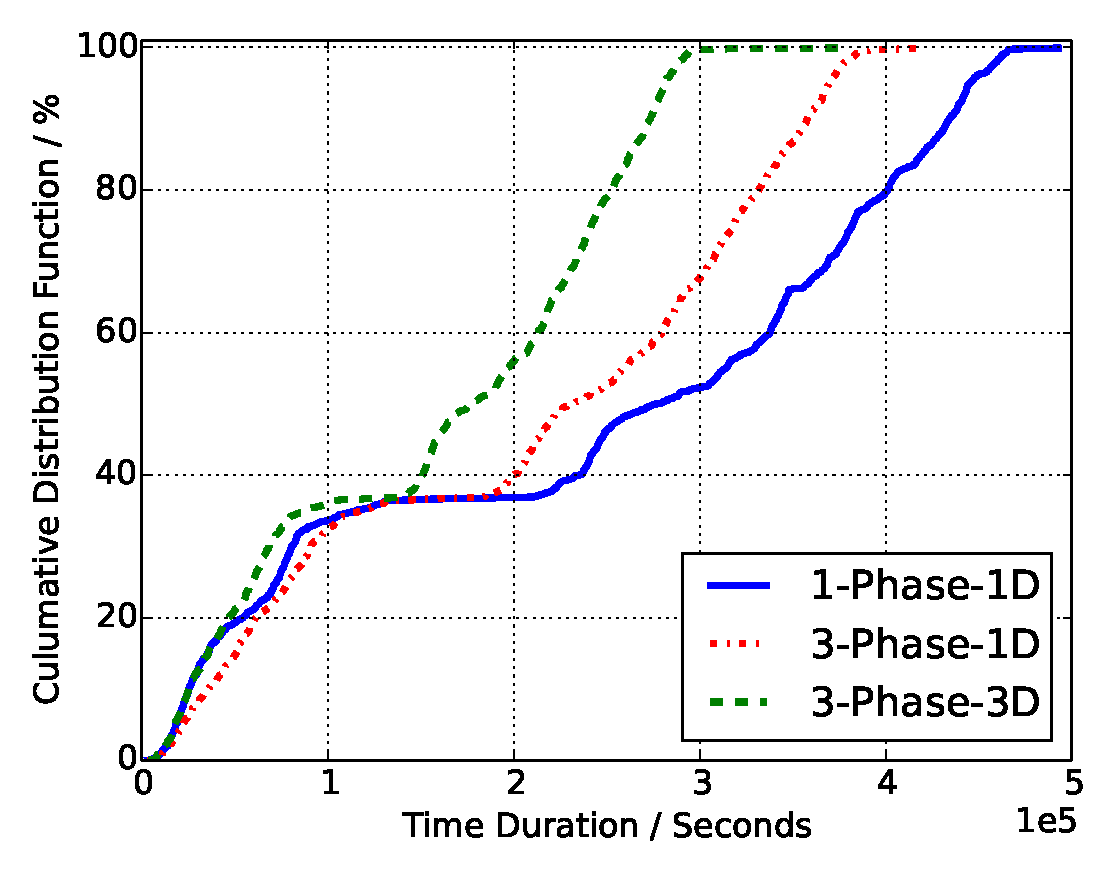
\includegraphics[width=2.2in]{3Pvs1PFigures/1000jobs_3p_vs_1p_response}
                \label{Fig:3Pvs1PResponse}
        }
        %\subfloat[Job Wait Time] {
                %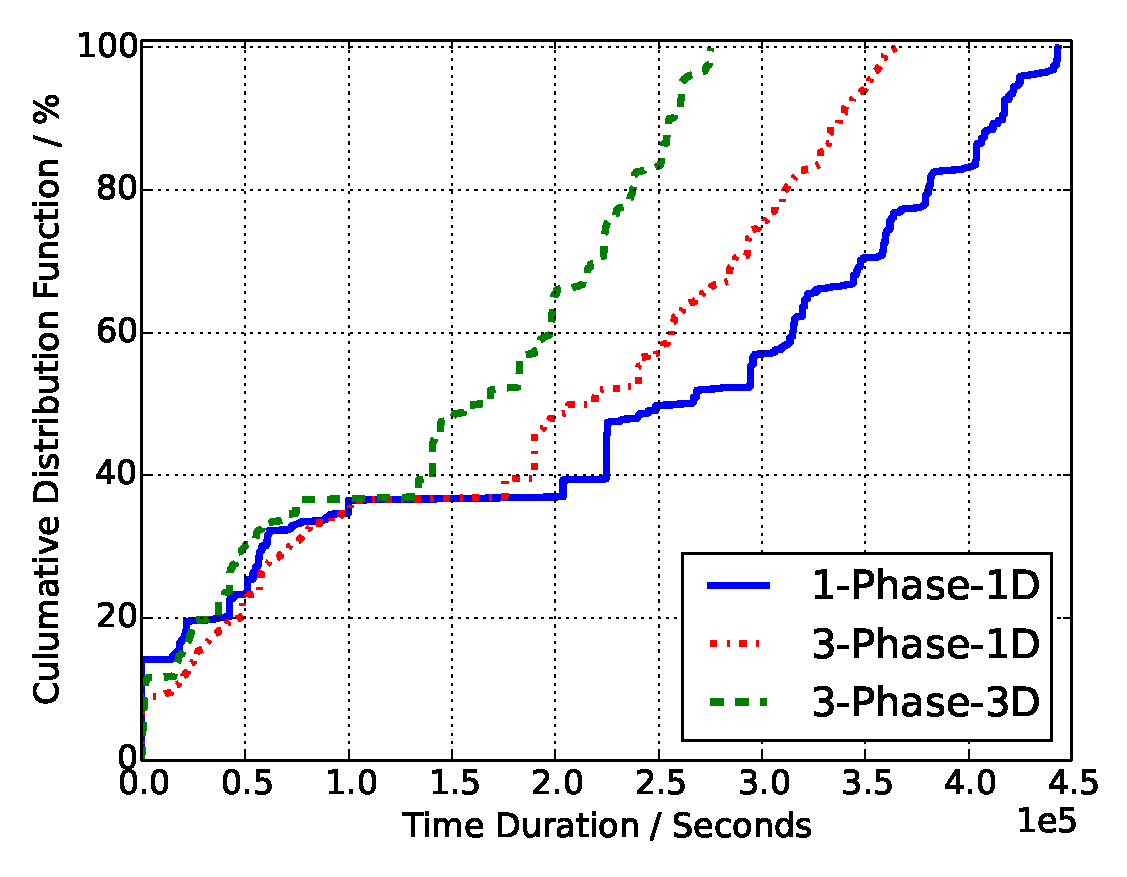
\includegraphics[width=3.2in]{3Pvs1PFigures/1000jobs_3p_vs_1p_wait}
                %\label{Fig:3Pvs1PWait}
        %}
        %\subfloat[Job Wait Input Time] {
                %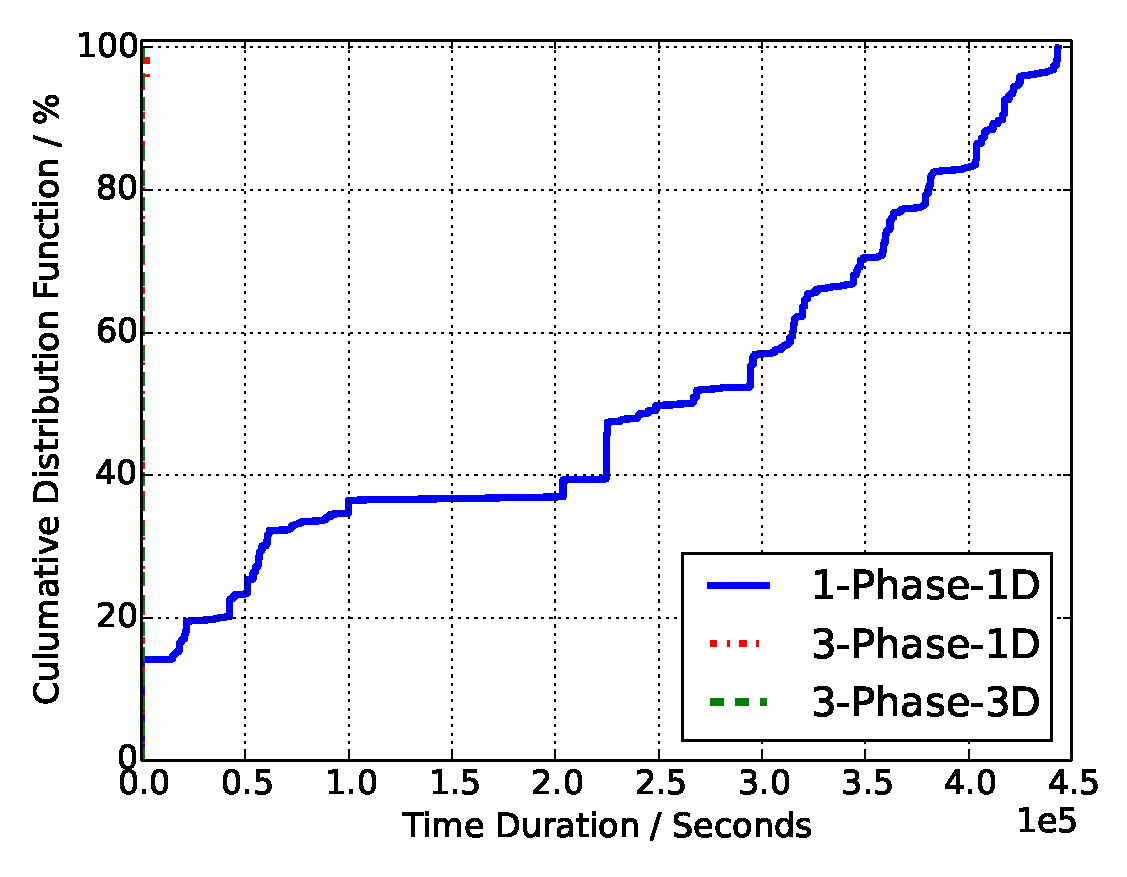
\includegraphics[width=2.3in]{3Pvs1PFigures/1000jobs_3p_vs_1p_wait_in}
                %\label{Fig:3Pvs1PWaitIn}
        %}
        %~
        \subfloat[Job Wait Run Time] {
                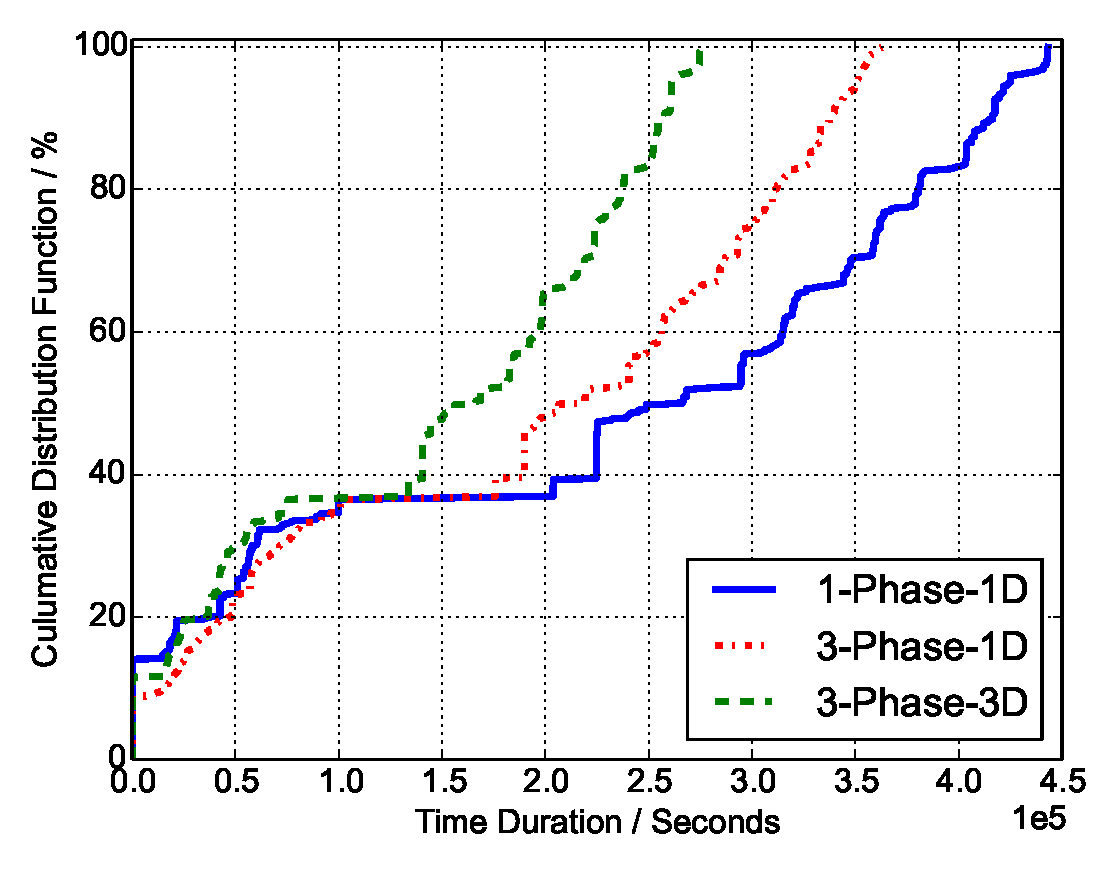
\includegraphics[width=2.2in]{3Pvs1PFigures/1000jobs_3p_vs_1p_wait_run}
                \label{Fig:3Pvs1PWaitRun}
        }
        \subfloat[System Throughput] {
                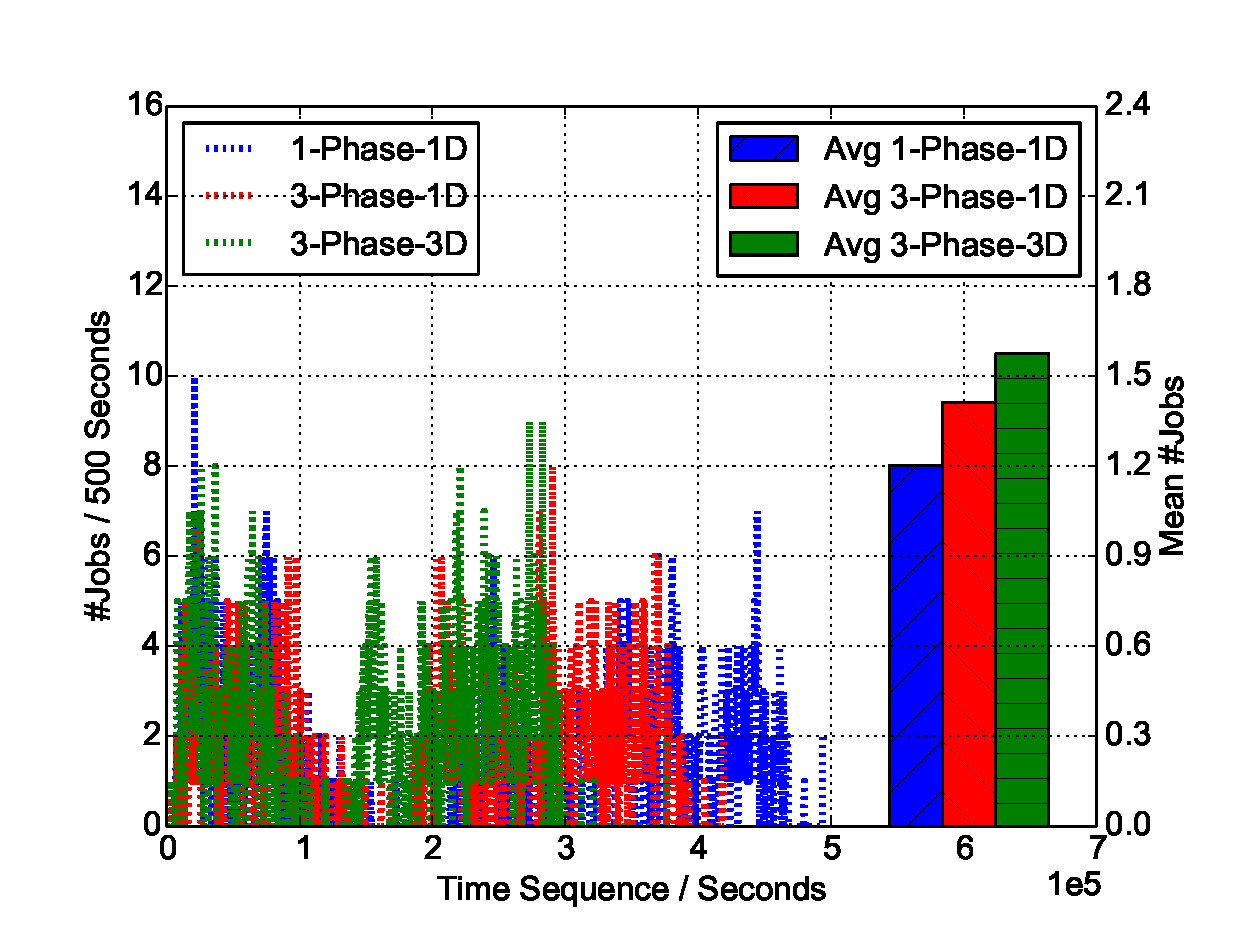
\includegraphics[width=2.5in]{3Pvs1PFigures/1000jobs_3p_vs_1p_throughput}
                \label{Fig:3Pvs1PThroughput}
        }
        \caption{3-Phase Model vs. 1-Phase Model}
        \label{Fig:3Pvs1PPerformance}
\end{figure*}

%\begin{figure}[!t]
        %\centering
        %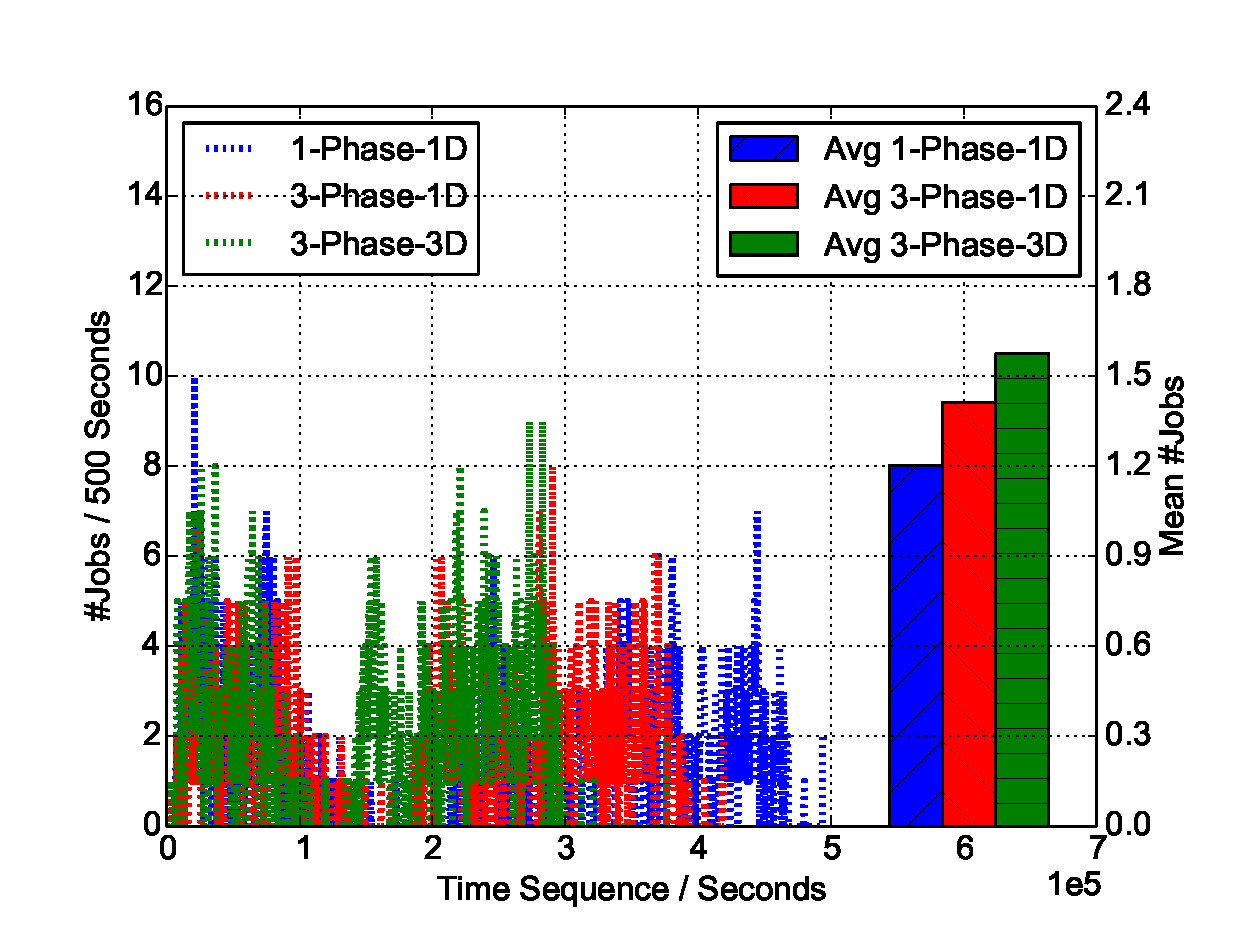
\includegraphics[width=3.2in]{3Pvs1PFigures/1000jobs_3p_vs_1p_throughput}
        %\caption{System Throughput, 1 Phase Model vs. 3 Phase Model}
        %\label{Fig:3Pvs1PThroughput}
%\end{figure}

\begin{figure*}[!t]
        \centering
        \subfloat[Job Response Time] {
                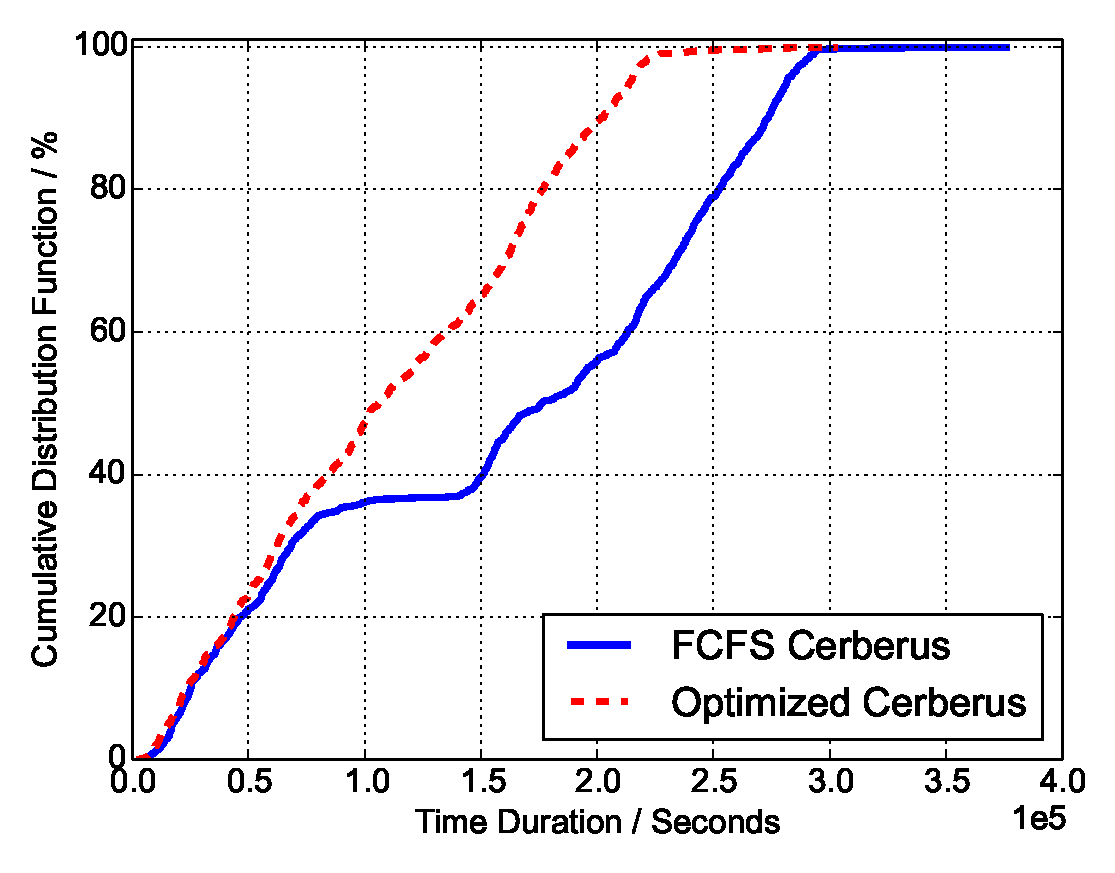
\includegraphics[width=2.2in]{DPvsFIFOFigures/1000jobs_dp_vs_fifo_response}
                \label{Fig:DPvsFIFOResponse}
        }
        \subfloat[Job Wait Run Time] {
                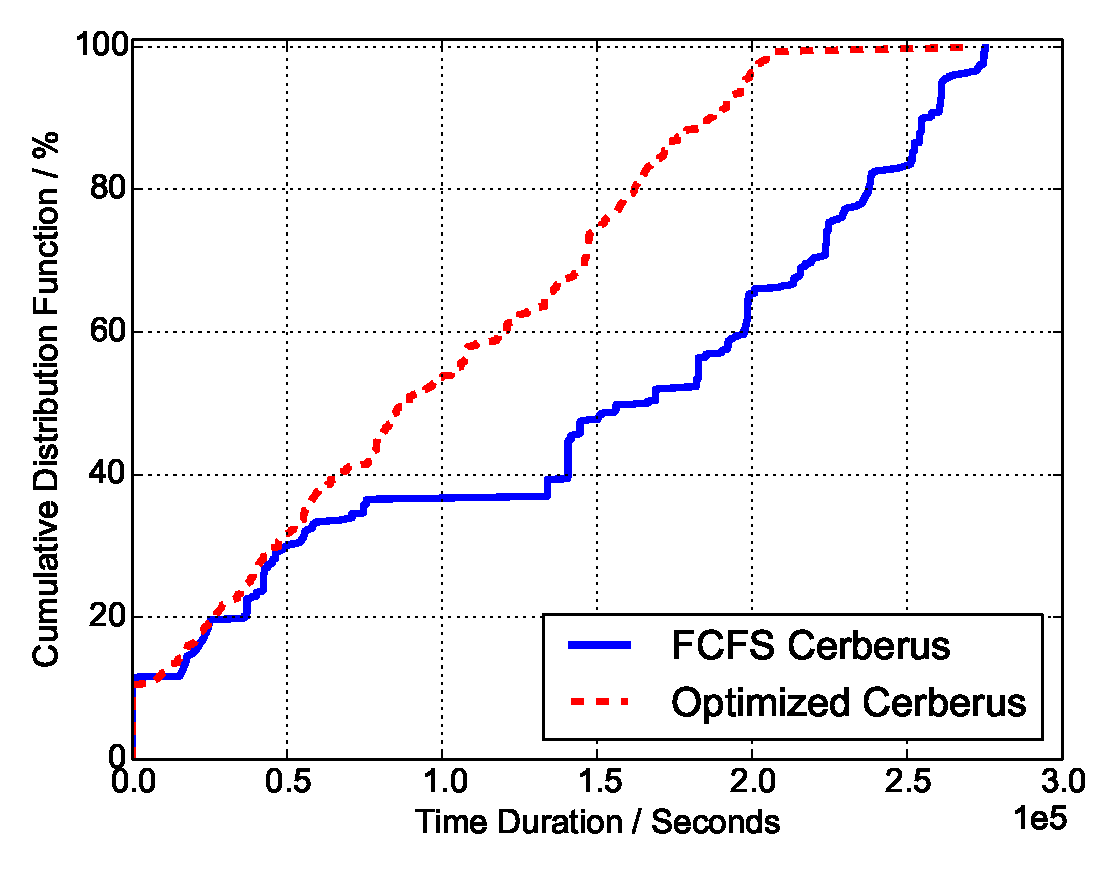
\includegraphics[width=2.2in]{DPvsFIFOFigures/1000jobs_dp_vs_fifo_wait_run}
                \label{Fig:DPvsFIFOWaitRun}
        }
        \subfloat[System Throughput] {
                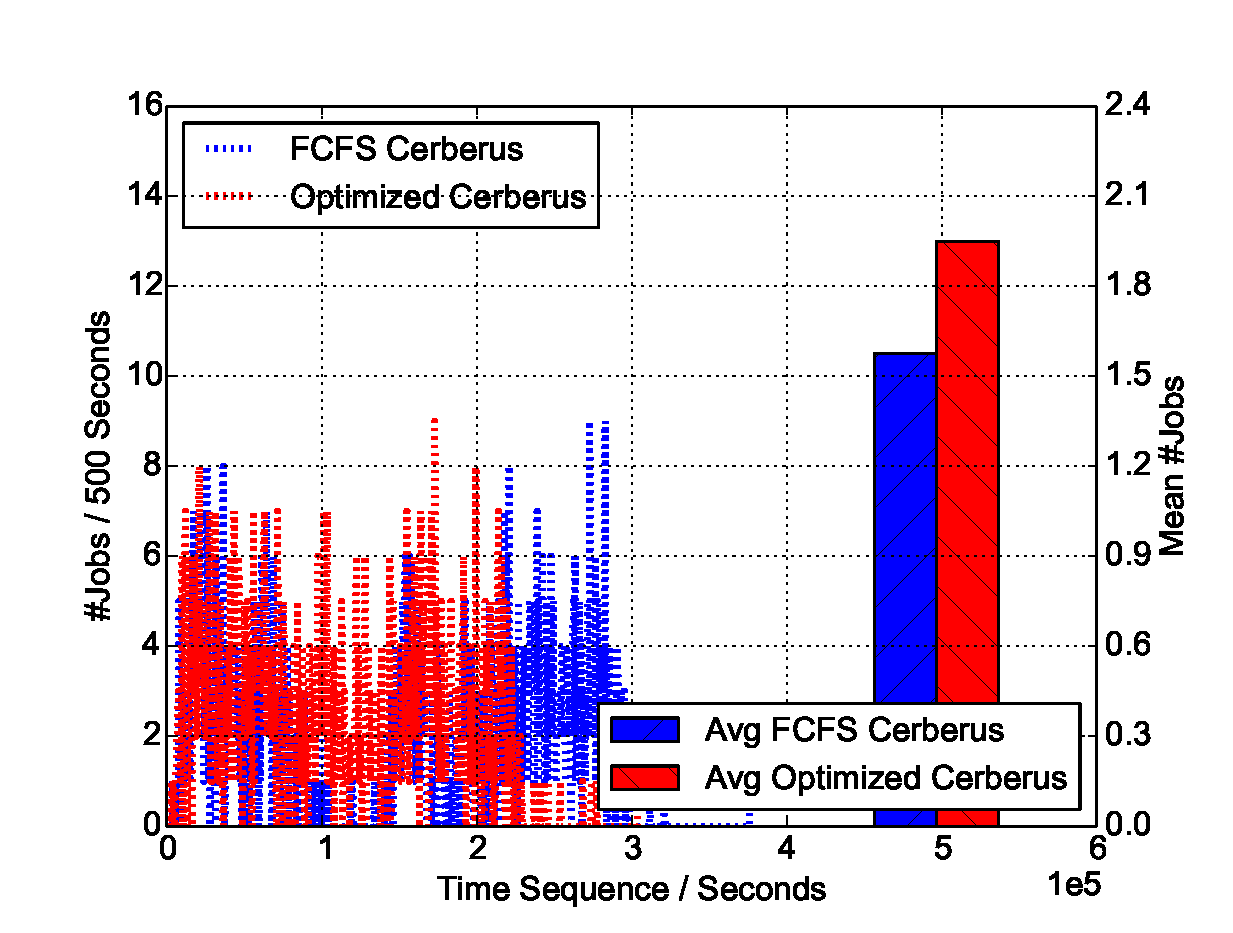
\includegraphics[width=2.5in]{DPvsFIFOFigures/1000jobs_dp_vs_fifo_throughput}
                \label{Fig:DPvsFIFOThroughput}
        }
        \caption{Optimized Cerberus v.s. FCFS Cerberus}
        \label{Fig:DPvsFIFOPerformance}
\end{figure*}

%\begin{figure}[!t]
        %\centering
        %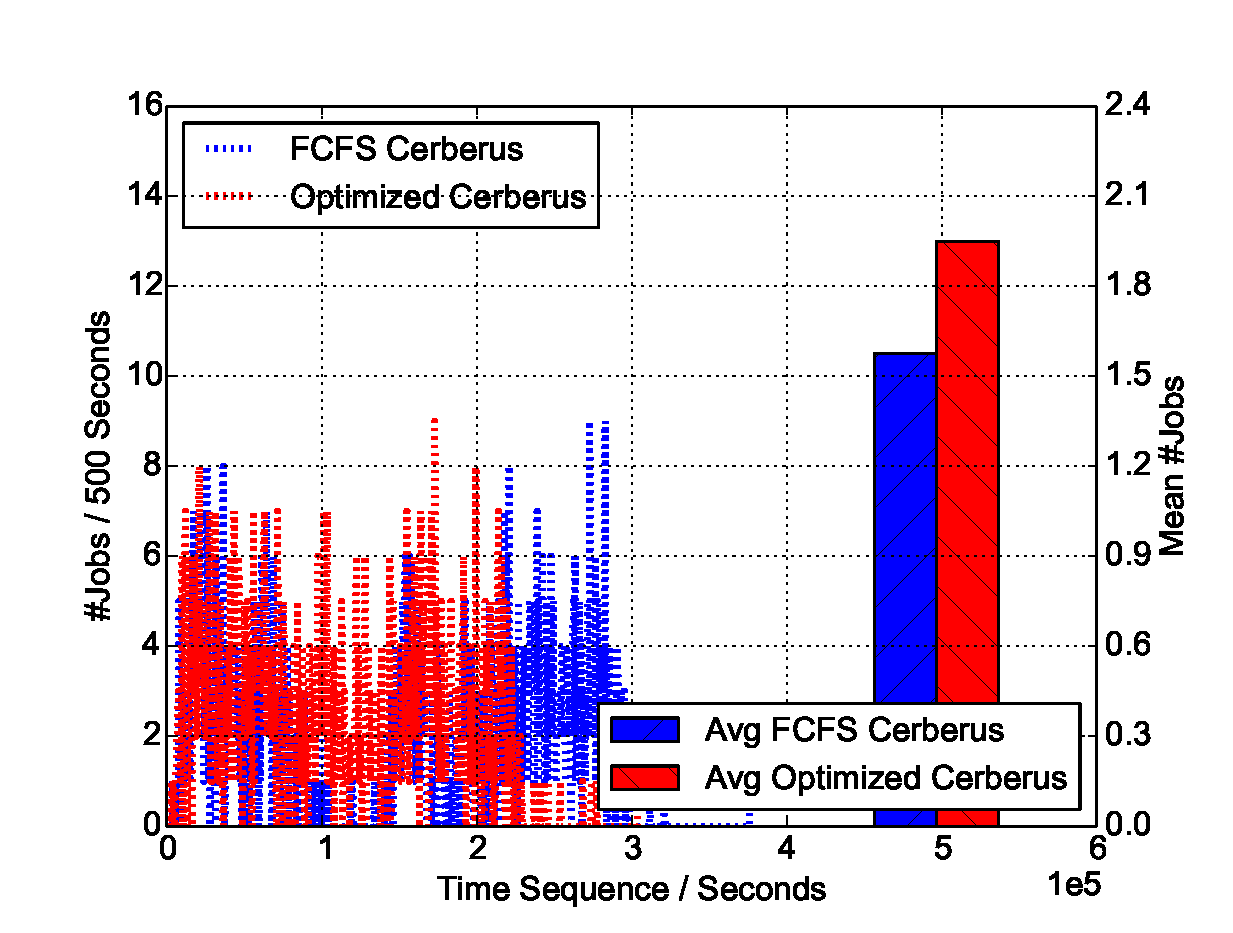
\includegraphics[width=3.2in]{DPvsFIFOFigures/1000jobs_dp_vs_fifo_throughput}
        %\caption{System Throughput, Optimized Cerberus vs. FCFS Cerberus}
        %\label{Fig:DPvsFIFOThroughput}
%\end{figure}

\subsection{Optimized Cerberus v.s. FCFS Cerberus}
%If we consider optimizing either burst buffer's data throughput or the parallelism across jobs,
%dynamic programming based job scheduler can further reduce jobs' wait time.
%We plot in Figure~\ref{Fig:DPvsFIFOResponse} the resulting response time of
%two versions of Cerberus:
%\begin{itemize}
%        \item \textbf{FCFS Cerberus} uses naive first come first serve policy.
%                Whoever at the front of queue are considered favorably.
%        \item \textbf{Optimized Cerberus} select these jobs in $Q_I$ and $Q_O$
%                such that volume of to be transferred data
%                is maximized by Recursion~\ref{Equ:MaxTransferDataRecursion}.
%                For jobs in $Q_R$, it chooses jobs according to the optimization solution
%                given by Equation~\ref{Equ:MaxProductRecursion}
%\end{itemize}
%As indicated by Figure~\ref{Fig:DPvsFIFOResponse}, response time of
%jobs scheduled by Optimized Cerberus is reduced.
%The most non-responsive job for Optimized Cerberus is job \#445,
%taking 303,523 seconds.
%In contrast, job \#445 takes 376,026 seconds to finish in FCFS Cerberus.
%This is 19.28\% slower than Optimized Cerberus.
%When we consider the overall response time of entire job set,
%we see more than \textit{80\% of the tasks response faster when we do optimization}.

%===========XY===============
In this section we answer question \textbf{Q3} by showing that
adopting optimizations in each scheduling phase brings further improvement,
comparing with the naive first come first server (FCFS) policy adopted in previous experiments.
Specifically, in the stage-in and stage-out phase, Cerberus schedules jobs in $Q_I$ and $Q_O$
according to solution given by \ref{Equ:MaxTransferDataRecursion};
for jobs in $Q_R$, Cerberus makes scheduling decision
based on the solution given by \ref{Equ:MaxProductRecursion}. %Algorithm~\ref{Alg:MaxCPU}.
We denote Cerberus coupled with two scheduling methodologies 
as \textbf{FCFS Cerberus} and \textbf{Optimized Cerberus} respectively.

As indicated by Figure~\ref{Fig:DPvsFIFOResponse}, response time of
jobs scheduled by Optimized Cerberus is reduced.
The most non-responsive job for Optimized Cerberus is job \#445,
taking 303,523 seconds.
In contrast, job \#445 takes 376,026 seconds to finish in FCFS Cerberus.
This is 19.28\% slower than Optimized Cerberus.
When we consider the overall response time of entire job set,
we see more than \textit{80\% of the tasks response faster when we do optimization}.


The time duration application waits for running,
or the time application spend in running queue,
is plotted in Figure~\ref{Fig:DPvsFIFOWaitRun}.
The tail of Optimized Cerberus shows that it holds a couple of jobs waiting
in its running queue for a very long time.
We figure out the reason of this long delay once we examine the detail of these jobs.
First they are submitted at early middle phase (job \#435 waits 268,322 seconds).
Second, these jobs are requesting huge amount (10240) of compute nodes
but comparably less burst buffer (7 TB for job \#435)
The third and the most important reason is that there are jobs requesting similarly
large number of cores but request less running time and larger amount of burst buffer.
For example, job \#434 requests 10240 compute nodes
but its expected running time is mere 3600 seconds;
in addition, it also requests 59 TB burst buffer.
As a result, Cerberus, according to \ref{Equ:MaxProductRecursion},
favors the jobs with less request time but larger burst buffer demand.
This is interesting because it is a potential flaws in the optimization-based policy:
given the user knows the optimization objective of our scheduler,
it is possible for a user to cheat scheduler by lying about her demand.
%In other words, our optimization scheme, even though providing performance enhancement
%for the waiting time of 70\% jobs, is not strategy-proofness\cite{Ghodsi:NSDI:2011}


We can see in Figure~\ref{Fig:DPvsFIFOThroughput} the system throughput
when scheduled by Cerberus with different scheduling objectives.
For optimized Cerberus, job \#445 decides the finishing time of all 1185 jobs.
That is 303,940 seconds for Optimized Cerberus.
FCFS Cerberus makes system ends its last job, also job \#455, at 376,443 seconds.
The worst case completion improvement to FCFS-style Cerberus is 19.26\%.
When we look at the time sequence of throughput,
we found the peak value 9 jobs / 500 seconds obtained by Optimized Cerberus.
The peak throughput of FCFS Cerberus is also 9 jobs / 500 seconds.
Mean throughputs of these 3 scheduling methods are drawn
as bar chart in Figure~\ref{Fig:DPvsFIFOThroughput}.
\textit{Comparing with FCFS Cerberus, Optimized Cerberus achieves
23.87\% higher average throughput (1.951 jobs / 500 seconds).}


%Table~\ref{Tab:OptimizationTime} demonstrate that 
% % Memoization technique helps optimized Cerberus be able to schedule jobs online,
% % though solving the optimization problem is theoretically NP-hard.
% % For Optimized Cerberus, it solved about 8400 Problem~\ref{Equ:MaxTransferData} and
% % Problem~\ref{Equ:MaxProduct} when scheduling all the jobs in workload,
% % taking less than 370 seconds.
% % The time overhead of solving each optimization is about 0.04 seconds per time.

%\begin{table}[!t] 
        %\renewcommand{\arraystretch}{1.3}
        %\caption{Time Consumption in Dynamic Programming}
        %\label{Tab:OptimizationTime}
        %\centering
        %\begin{tabular}{l|c}
                %\hline
                %Optimization Policy Used & Optimized Cerberus\\
                %\hline
                %\hline
                %Simulation Run Time / seconds & 375.55\\
                %Optimization Run Time / seconds & 364.62\\
                %Total Number of Optimizations & 8406\\
                %\hline
        %\end{tabular}
%\end{table}

Memoization technique helps optimized Cerberus be capable to schedule jobs online,
though solving the optimization problem is theoretically NP-hard.
In our simulation, it takes averagely about 0.04 second for the optimized 
Cerberus to make one scheduling decision.


